\documentclass{article}
\usepackage[utf8]{inputenc}


\title{Iron toxicity text experiment }
\author{Jincheng Han}
\date{October 2018}

\usepackage{natbib}
\usepackage{graphicx}
\usepackage{multirow}
\usepackage{longtable}
\usepackage{booktabs}
\usepackage{tabu}
\newcommand{\head}[1]{\textnormal{\textbf{#1}}}

\begin{document}

\maketitle

\section{Objective  }
Iron toxicity test for perchlorate reduction bacteria
\section{Hypothesis }
The presence of ferrous and ferric iron will inhibit the growth of perchlorate bacteria. (the effect of ferrous iron will be more significant). 
\section{Methods }

\begin{center}
\begin{longtable}{|c|c|c|}
\caption{enrichment culture.} \label{tab:long} \\
\hline \multicolumn{1}{|c|}{\textbf{compounds}} & \multicolumn{1}{c|}{\textbf{concentration }} & \multicolumn{1}{c|}{\textbf{volume }} \\ \hline 
\endfirsthead

\multicolumn{3}{c}%
{{\bfseries \tablename\ \thetable{} -- continued from previous page}} \\
\hline \multicolumn{1}{|c|}{\textbf{First column}} & \multicolumn{1}{c|}{\textbf{Second column}} & \multicolumn{1}{c|}{\textbf{Third column}} \\ \hline 
\endhead

\hline \multicolumn{3}{|r|}{{Continued on next page}} \\ \hline
\endfoot

\hline \hline
\endlastfoot

media solution  & --- & 1000ml \\
Bacteria  & --- & 100ml \\
Perchlorate (from the stock) & 100,000 mg/l  & 10ml \\
Ethanol & 1000 mg & 1.25ml \\


\end{longtable}
\end{center}

\begin{itemize}
\item Enrichment culture 
\end{itemize}
Media solution follows Bruce 1999, including fresh medium, vitamin and trace element. Add media solution, bacteria, perchlorate stock and ethanol following the table 1.Culture the bacteria in the dark room, $25^\circ$C, 80rpm/mins. In the meantime, sample the perchlorate concentration every 48h until the perchlorate concentration is almost 0mg/l. All operation is under the anaerobic condition.
\begin{itemize}
\item PIPES Buffer 
\end{itemize}

Making 20mM PIPES buffer and adjust pH under $N_{2}$-C$O_{2}$ head-space for 20mins to make sure no oxygen in the PIPES buffer.Growth cultures were conducted using freshwater 30mM bicarbonate-buffered basal media (pH 6.8) under a N2-CO2 (80\%:20\%) headspace. During this experiment, there are 3 repeats. Washed cell suspensions were carried out by centrifuging 200mL of cells grown in minimal media and washing twice with 20mM PIPES buffer, pH 7, and re-suspending after a third centrifuging in the same buffer.	Added 2ml perchlorate from perchlorate stock and 0.25ml ethanol from stock. Measured main parameters every 6h.
\begin{itemize}
\item Different Treatment 
\end{itemize}

\centering
\begin{tabular}{c|c|c|c|c|c}

     & IT1& IT2& IT3& IT4& IT5 \\
     \hline 
      & positive control & negative control &2mM $Fe^{2+}$& 2mM $Fe^{3+}$& $Fe^{2+}$+$Fe^{3+}$\\
     PIPES Buffer& 198.15ml& 196.4ml& 196.5ml& 196.5ml& 196.5ml\\PIPES Perchlorate & 1.6ml& 1.6ml&1.6ml& 1.6ml& 1.6ml\\
     Ethanol & 0.25ml& --- & 0.25ml& 0.25ml& 0.25ml\\
     $Fe^{2+}$ & ---& 2ml&2ml& ---ml& 1ml\\
     $Fe^{3+}$ &---& ---&---& 2ml& 1ml\\
    
     
\end{tabular}

\section{methond}
i like you 
\textbf{}
\begin{figure}[h!]
\centering
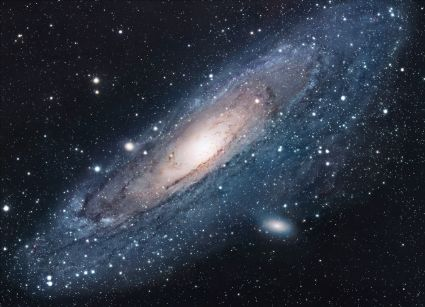
\includegraphics[scale=1.7]{universe}
\caption{The Universe}
\label{fig:universe}
\end{figure}

\section{Conclusion}
``I always thought something was fundamentally wrong with the universe'' \citep{adams1995hitchhiker}

\bibliographystyle{plain}
@article{bruce1999reduction,
  title={Reduction of (per) chlorate by a novel organism isolated from paper mill waste},
  author={Bruce, Royce A and Achenbach, Laurie A and Coates, John D},
  journal={Environmental microbiology},
  volume={1},
  number={4},
  pages={319--329},
  year={1999},
  publisher={Wiley Online Library}
}
\bibliography{references}

\end{document}
